\section{Fitting}
\label{sec:fitting}
This section will fit Model $\mathcal{A}$ using Synthetic Likelihood Estimation. Since Model $\mathcal{A}$ is quite complicated, this section will start by looking at a simplified model where there is no regime switching. Fitting this simplified model will provide the building blocks to fit Model $\mathcal{A}$.

To start with, synthetic data will be used instead of real data. A sample can be drawn using fitted values  for the UK power data (Table~\ref{tab:uk-val}) from \cite{huisman_mahieu_2003}. This sample will be used as the observed trajectory which will then be used to fit the model. This allows for a comparison between the fitted parameters and the original parameters to check the statistics properly explain the dynamics of the model.

In Section \ref{subsec:fit-real}, historic data from Nordpool will be used to fit the model.

\subsection{Fitting a Simplified Model (Model \texorpdfstring{$\mathcal{B}$}{B})}
The cleanest way to simplify Model $\mathcal{A}$ is to forget the regime-switching part and stay in regime $0$ for all time. This means the simplified model is specified as follows. Model the natural log of the spot price $s(t)$ as the sum of the deterministic component $f(t) = \mu_0 + \beta_1 D_1(t) + \beta_2 D_2(t)$ and the stochastic component $x(t)$. However, the stochastic component is now modelled as $x(1) = 0$ and
\begin{equation}
    \dif{x(t)} = x(t) - x(t-1) = -\alpha_0 x(t-1) + \sigma_0 \epsilon_t
\end{equation}
for $t > 1$. Constrained parameters $\alpha_0$ and $\sigma_0$ still need to be replaced with unconstrained parameters $\tau_{\alpha_0}$ and $\tau_{\sigma_0}$ as per Section~\ref{subsec:constr-par}. Call the above model, Model $\mathcal{B}$.

\subsubsection{Choice of Statistics}

Now, the statistics need to be chosen. For $\mu_0$ and $\sigma_0$, include the Maximum Likelihood Estimates from a Normal distribution. Denote the sample mean as $\bar{x}(\cdot)$ and standard deviation as $\sd{(\cdot)}$. Additionally, $\beta_1$ and $\beta_2$ represent the price increment on a Saturday and a Sunday respectively. Thus, to infer these parameters, include the mean price on a Saturday, denoted as $\bar{x}_5(\cdot)$, and on a Sunday, denoted as $\bar{x}_6(\cdot)$. Notice, Monday is considered day $0$, so Saturday is day $5$ and Sunday is day $6$ in this notation. Finally, statistics are needed for $\alpha_0$, the mean-reversion parameter. There are a few statistics that may be useful. First, mean-reversion is to do with the relationship between $x(t)$ and $x(t-1)$. Thus, it would make sense to include autocorrelation coefficients. However, these are not $M$-estimators. Taking a closer look at the dynamics of Model $\mathcal{B}$ reveals a similar option - autoregression coefficients. Expanding the Model $\mathcal{B}$ yields
\begin{align}
    s(t) &= f(t) + x(t) \\
    &= f(t) + x(t-1) + \dif{x(t)} \\
    &= f(t) + x(t-1) - \alpha_0 x(t-1) + \sigma_0 \epsilon_t \\
    &= f(t) + (1-\alpha_0)x(t-1) + \sigma_0 \epsilon_t \\
    &= f(t) + (1-\alpha_0)(s(t-1) - f(t-1)) + \sigma_0 \epsilon_t \\
    &= f(t) + (1-\alpha_0)f(t-1) + (1-\alpha_0)s(t-1) + \sigma_0 \epsilon_t.
\end{align}

The expanded dynamics show that an autoregression of the form
\begin{equation}
    s(t) \approx \xi_0 + \xi_1 s(t-1)
\end{equation}
is appropriate, with the gradient parameter, $\xi_1$, of particular interest. Since OLS estimators, denoted $\xi_0(\cdot)$ and $\xi_1(\cdot)$ respectively, are $M$-Estimators as per proposition~\ref{prop:ols}, all the statistics are $M$-Estimators. Thus, Synthetic Likelihood Estimation can be compared with and without using the Robust Covariance Matrix. Before proceeding, the correlation diagrams defined in Section~\ref{subsec:corr_diag} will be computed.

These are shown in Figure~\ref{fig:smcd}. Each parameter is reasonably correlated with one of the statistics and the statistics themselves are not too correlated. There are two classes of notable correlation between the statistics. The first is between the mean spot price, the mean spot price on Saturday and the mean spot price on Sunday. This could be fixed by subtracting the mean from the mean on Saturday and the mean Sunday, but the resulting statistics would no longer be $M$-Estimators. The other area of notable correlation is between $\xi_1$ and $\xi_2$, the autoregression intercept and gradient. This correlation is expected since both parameters are strongly correlated with $\alpha_0$. Both statistics need to be included in order to use the Robust Covariance Matrix.

\begin{figure}[H]
        \centering
        \subfloat{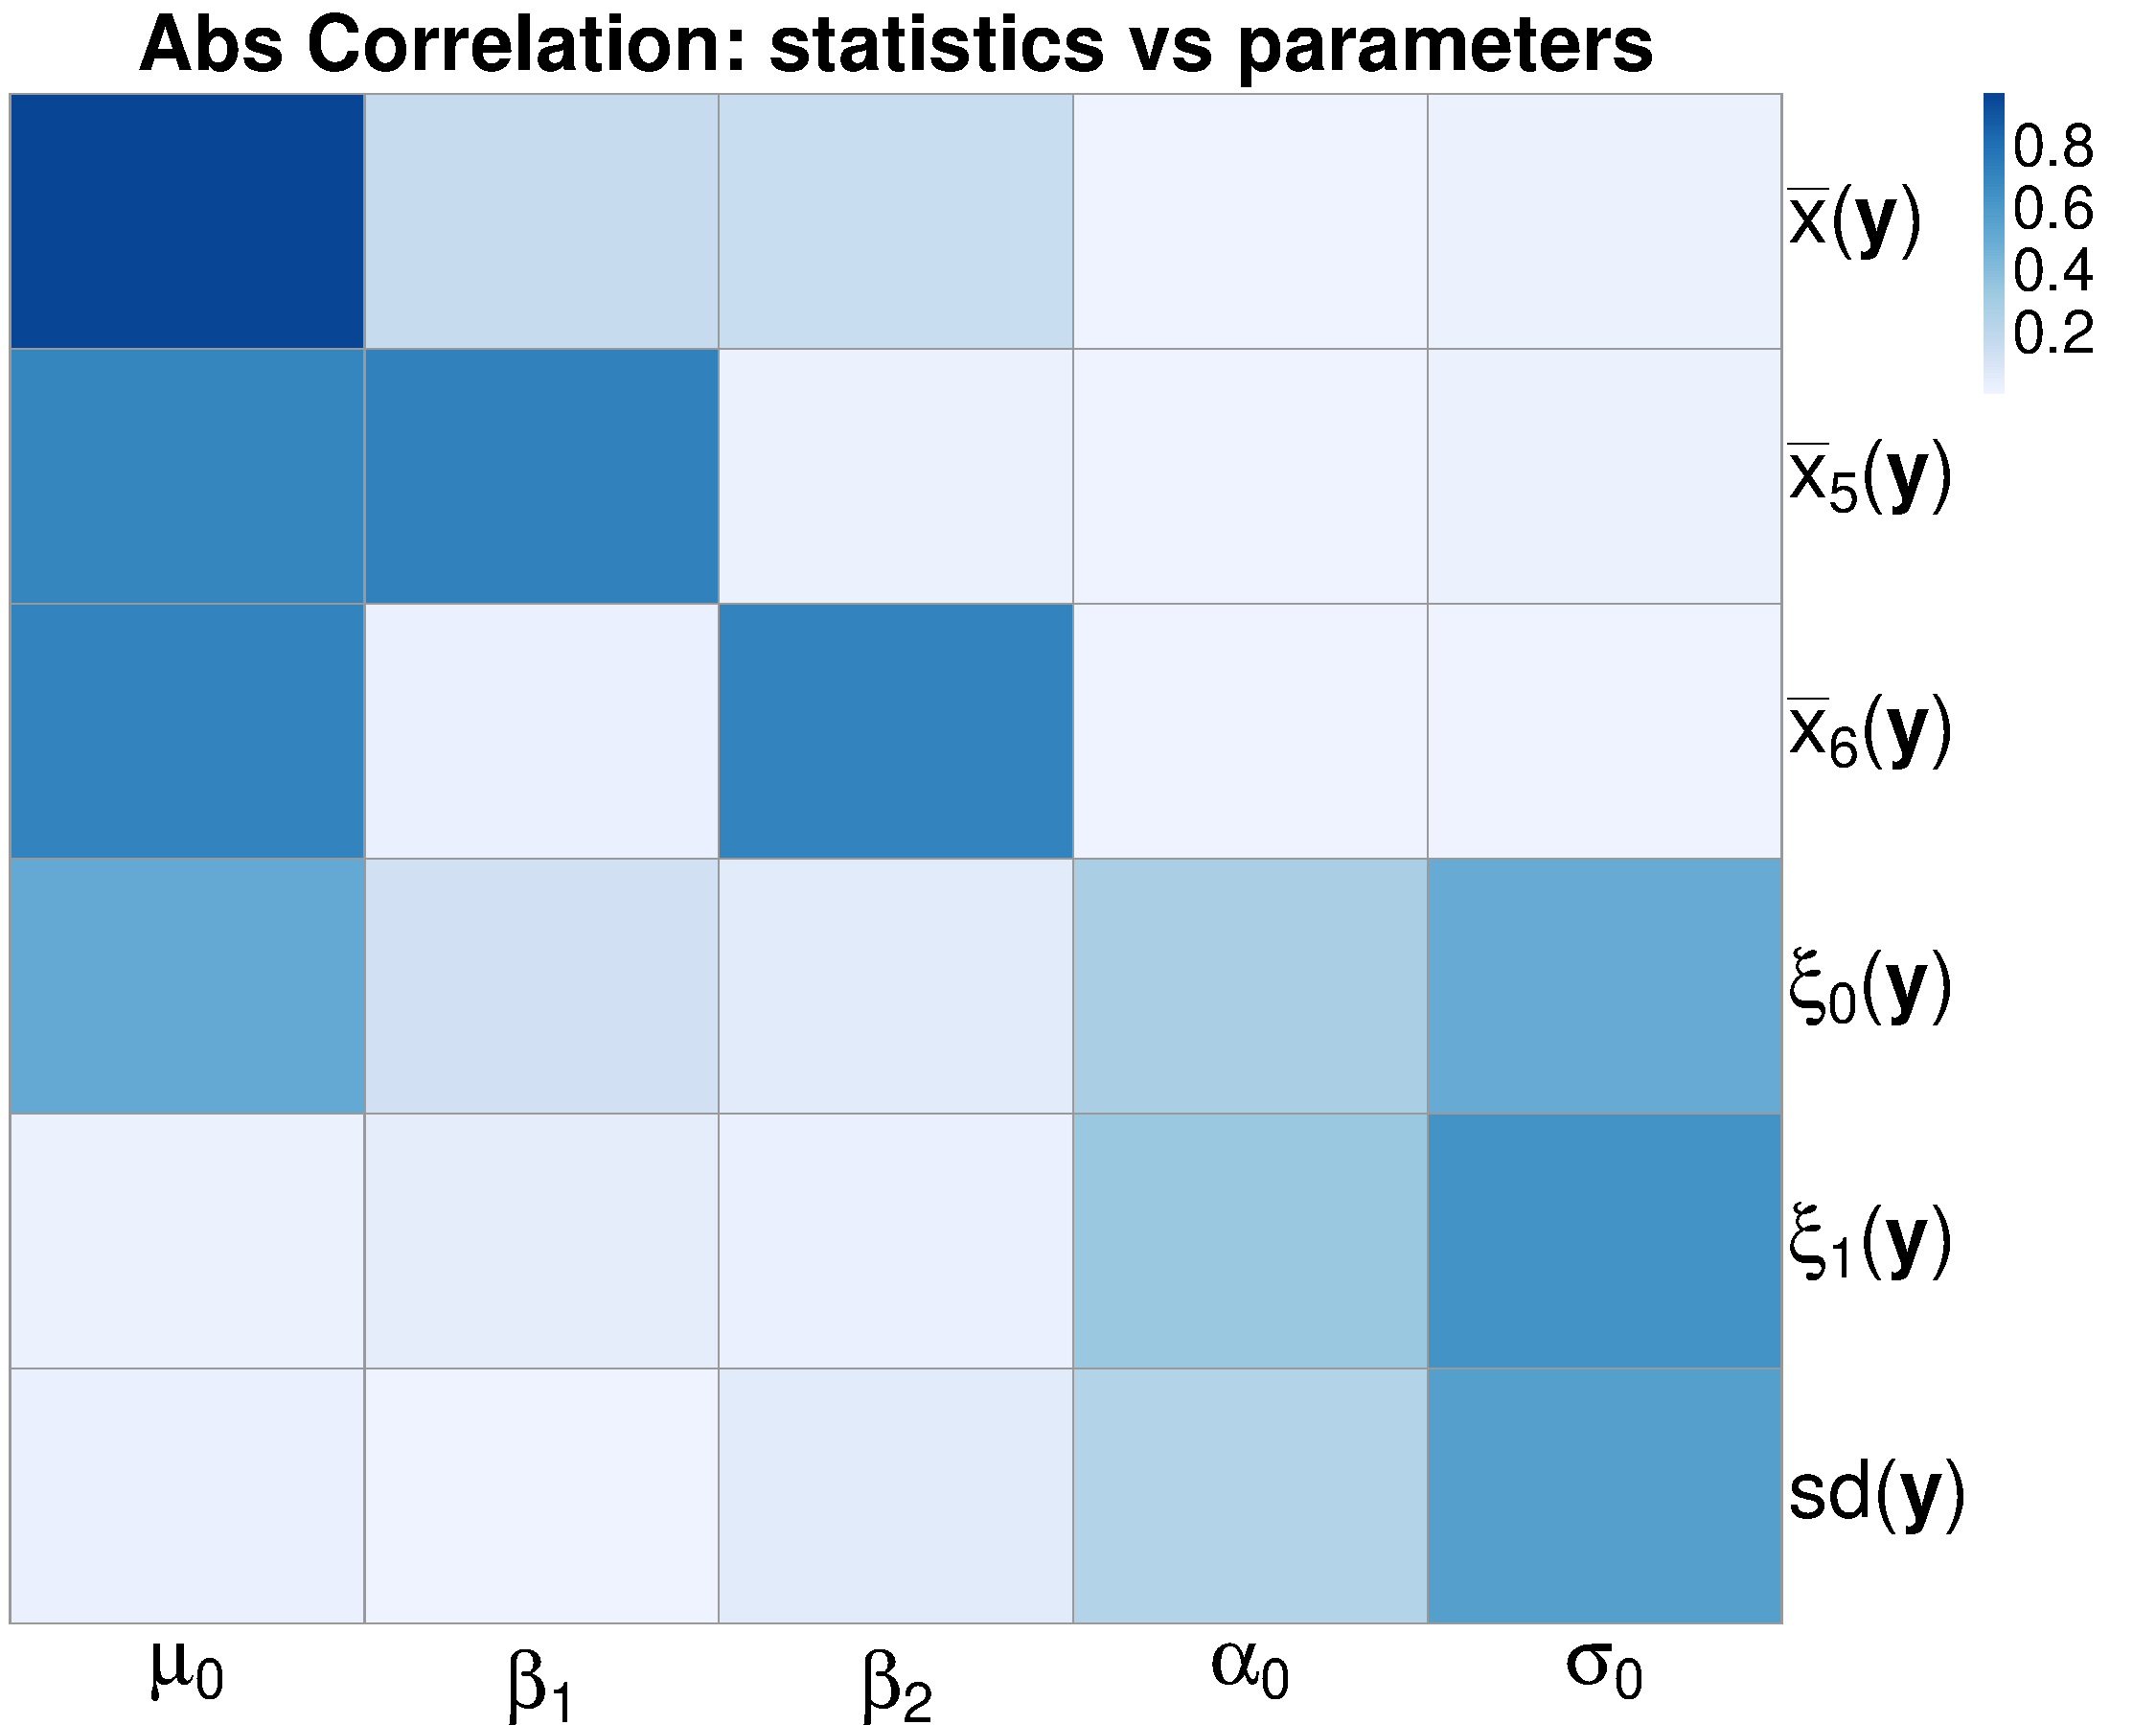
\includegraphics[width=55mm]{images/fitting/simple_model/cor_sp.pdf}}
        \qquad
        \subfloat{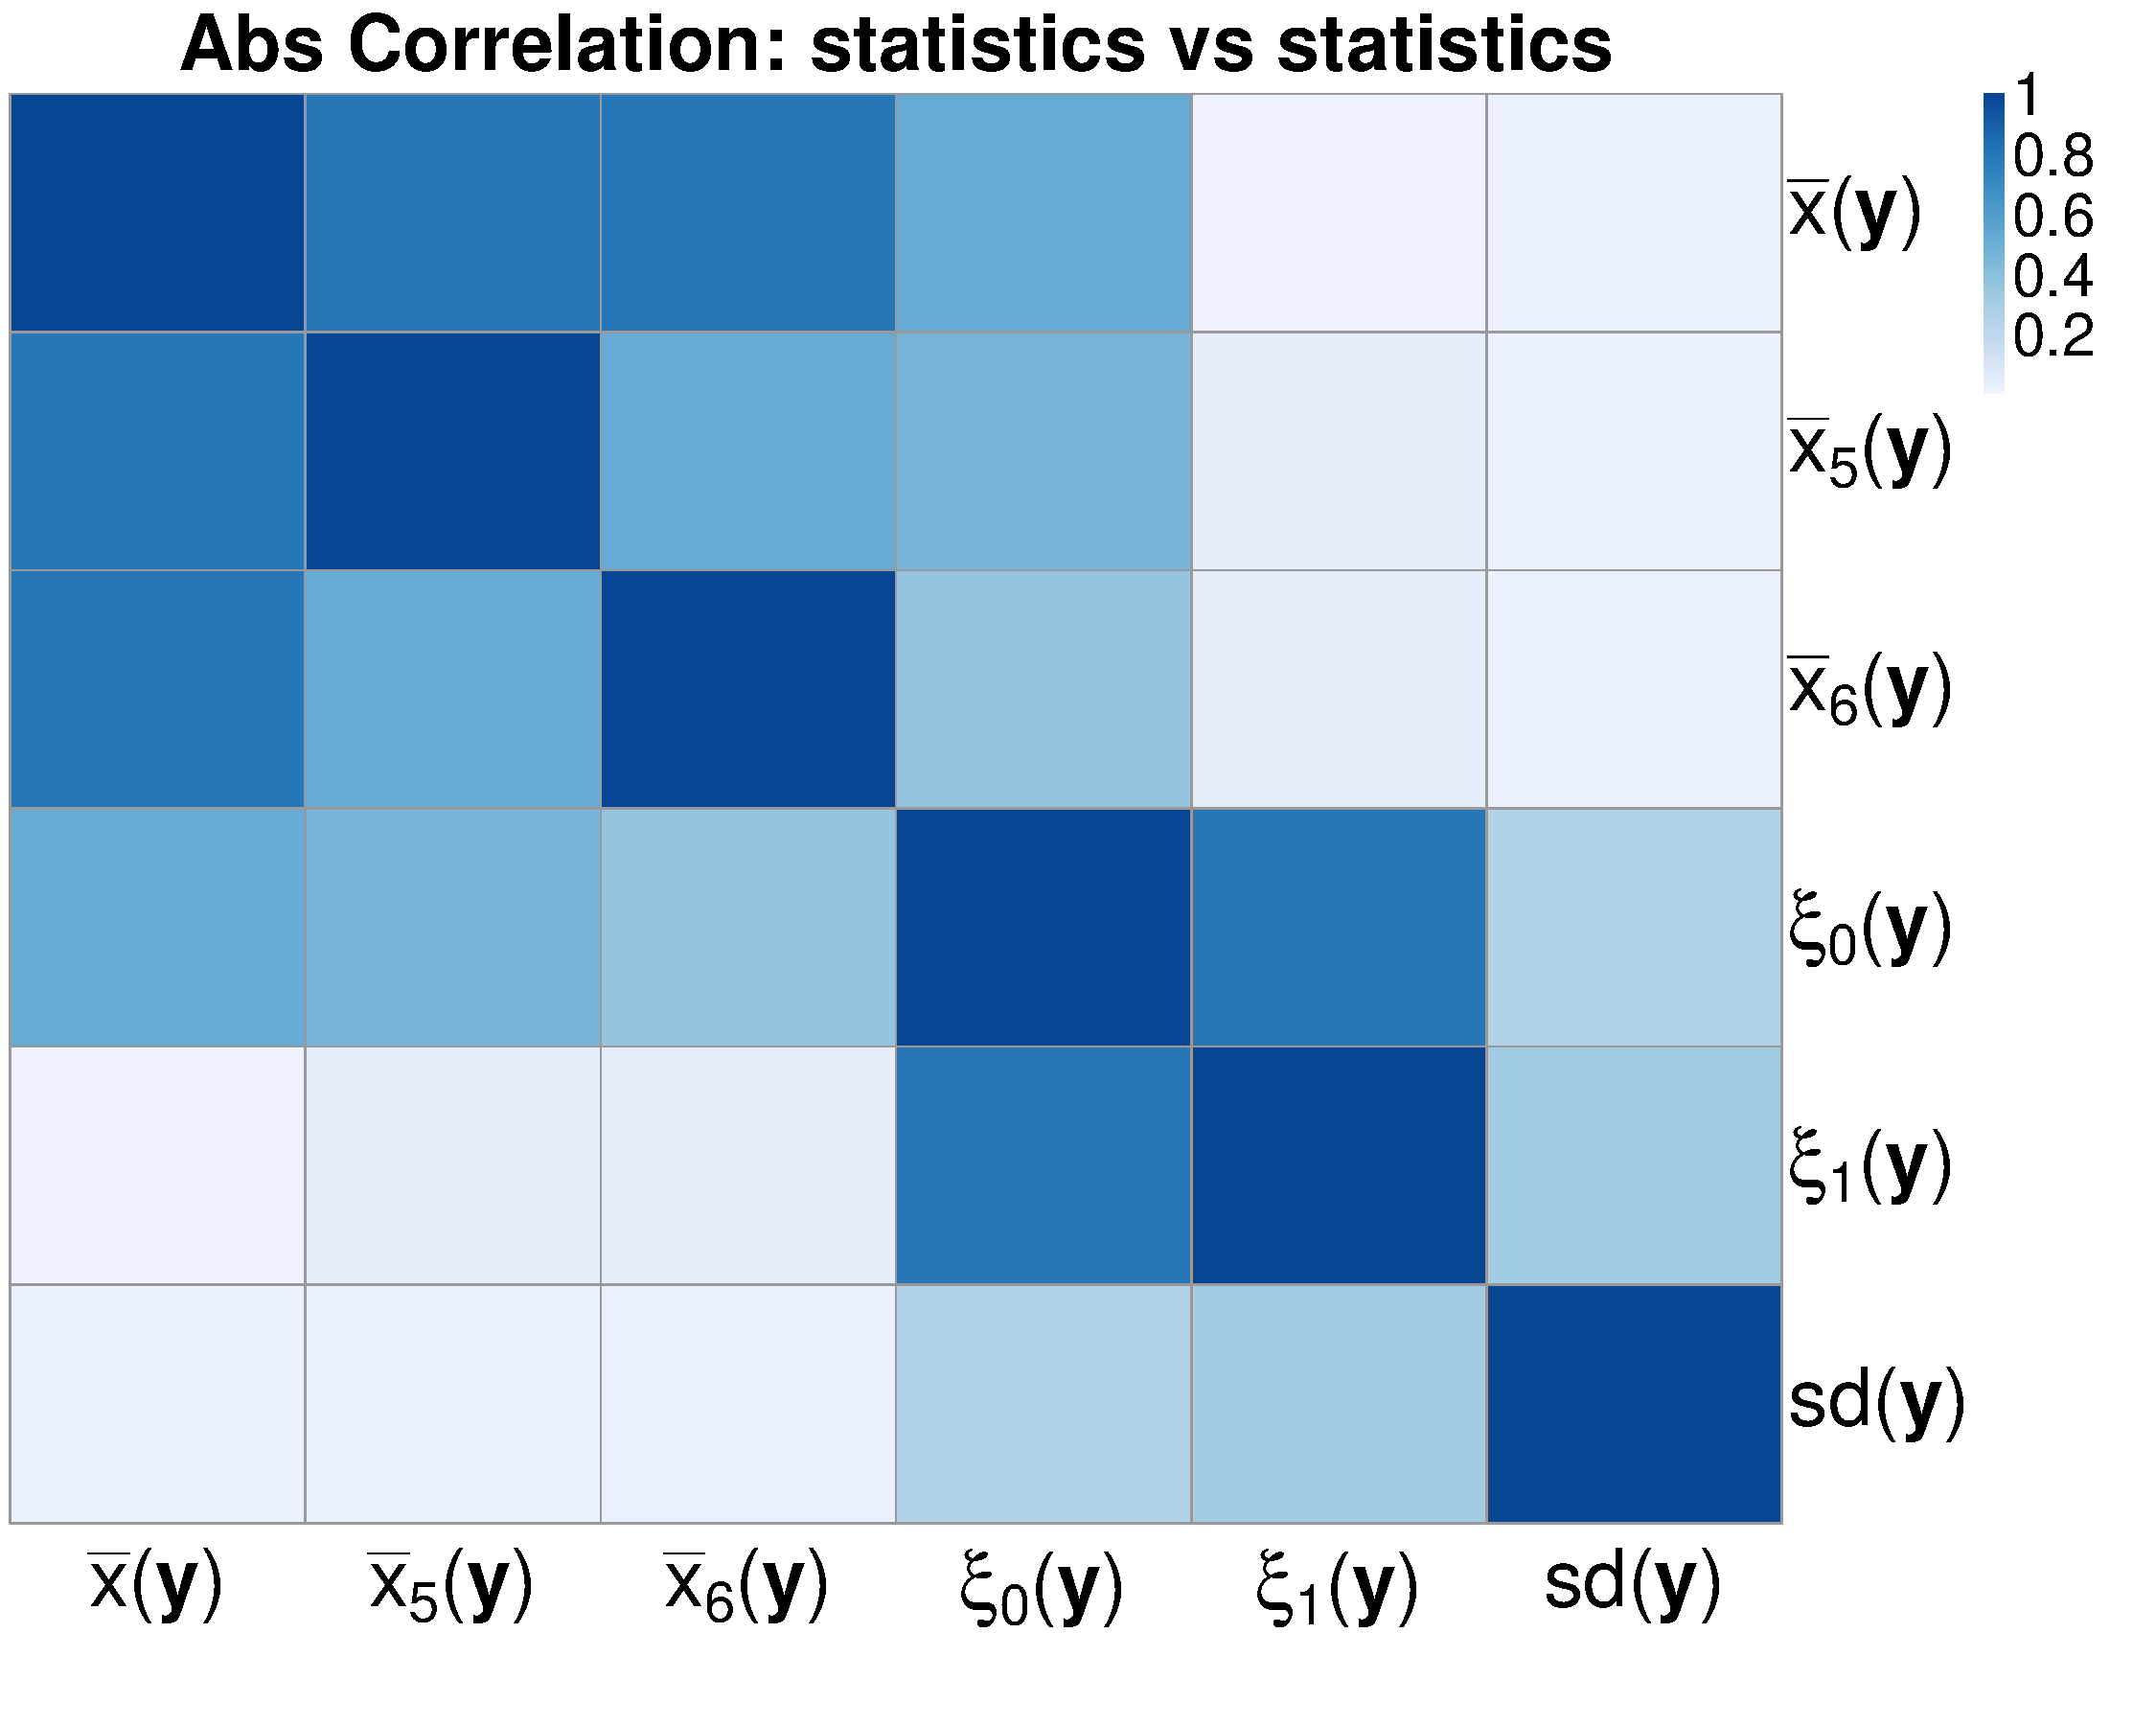
\includegraphics[width=55mm]{images/fitting/simple_model/cor_ss.pdf}}
        \caption{Model $\mathcal{B}$ Correlation Diagrams}
        \label{fig:smcd}
\end{figure}

In order to compute the Robust Covariance Matrix, a loss function is needed. Let $m$ be the observation length and $\pmb{y}^0$ the observed trajectory. A sample trajectory $\pmb{y}^1$ is also needed which the statistics will be evaluated along. For $\bar{x}(\cdot)$ and $\sd{(\cdot)}$, the negative log-likelihood of a Normal distribution will suffice. Write
\begin{equation}
    L_{1,2} = -\sum_{i=1}^m \log{f(y^1_i | s_1, s_2^2)}
\end{equation}
where $f$ is the density of a Normal random variable with mean $s_1 = \bar{x}(\pmb{y}^1)$ and standard deviation $s_2 = \sd{(\pmb{y}^1})$.

Now, for $\bar{x}_5(\cdot)$ and $\bar{x}_6(\cdot)$, the mean price on a Saturday and a Sunday respectively. Here, a quadratic loss function will be used. That is,
\begin{equation}
    L_3 = \frac{1}{2}\sum_{i=1}^m (s_3 - y^1_i)^2 \mathbb{I}\{i \equiv 5 \Mod{7}\}
\end{equation}
and
\begin{equation}
    L_4 = \frac{1}{2}\sum_{i=1}^m (s_4 - y^1_i)^2 \mathbb{I}\{i \equiv 6 \Mod{7}\}
\end{equation}
where $s_3 = \bar{x}_5(\pmb{y}^1)$ and $s_4 = \bar{x}_6(\pmb{y}^1)$.

Finally, for the OLS regression estimators, the sum of squared residuals loss function will be used. Write
\begin{equation}
    L_{5,6} = \sum_{i=2}^m [y^1_i - (s_5 + s_6 y^1_{i-1})]^2
\end{equation}
where $s_5 = \xi_0(\pmb{y}^1)$ and $s_6 = \xi_1(\pmb{y}^1)$.

These individual loss functions can now be summed to obtain a loss function for the vector of statistics $\pmb{s} = (s_1, \ldots, s_6)$. Concretely,
\begin{equation}
    \begin{split}
        L &= -\sum_{i=1}^m \log{f(y^1_i | s_1, s_2^2)} + \frac{1}{2}\sum_{i=1}^m (s_3 - y^1_i)^2 \mathbb{I}\{i \equiv 5 \Mod{7}\} \\ &+ \frac{1}{2}\sum_{i=1}^m (s_4 - y^1_i)^2 \mathbb{I}\{i \equiv 6 \Mod{7}\} + \sum_{i=2}^m [y^1_i - (s_5 + s_6 y^1_{i-1})]^2.
    \end{split}
\end{equation}

The next step is to compute the gradient and Hessian of $L$. The gradient turns out to be
\begin{equation}
    (\nabla L(\pmb{s}))|_{y_i} =
    \begin{pmatrix}
        - \frac{y^1_i - s_1}{s_2^2} \\
        \frac{s_2^2 - (y^1_i - s_1)^2}{s_2^3} \\
        (s_3 - y^1_i)\mathbb{I}\{i \equiv 5 \Mod{7}\} \\
        (s_4 - y^1_i)\mathbb{I}\{i \equiv 6 \Mod{7}\} \\
        2(-y^1_i + y^1_{i-1}s_6 + s_5)\mathbb{I}\{i > 1\} \\
        2y^1_{i-1}(-y^1_i + y^1_{i-1}s_6 + s_5)\mathbb{I}\{i > 1\}
    \end{pmatrix}.
\end{equation}

To achieve the greatest computational benefit from using the Robust Covariance Matrix, the Hessian will also be computed analytically. This is just a matter of further differentiating the gradient. It is also possible to compute the Hessian numerically; this will
be considered for the performance section (Section \ref{subsec:perf}). For the analytic Hessian, obtain
\begin{equation}
    \pmb{H}_L(\pmb{s}) = \sum_{i=1}^m \scalemath{0.65}{\begin{pmatrix}
        \frac{1}{s_2^2} & \frac{2(y^1_i - s_1)}{s_2^3} & 0 & 0 & 0 & 0 \\
        \frac{2(y^1_i - s_1)}{s_2^3} & -\frac{1}{s_2^2} + \frac{3(y^1_i -s_1)^2}{s_2^4} & 0 & 0 & 0 & 0 \\
        0 & 0 & \mathbb{I}\{i \equiv 5 \Mod{7}\} & 0 & 0 & 0 \\
        0 & 0 & 0 & \mathbb{I}\{i \equiv 6 \Mod{7}\} & 0 & 0 \\
        0 & 0 & 0 & 0 & 2\mathbb{I}\{i > 1\} & 2y^1_{i-1}\mathbb{I}\{i > 1\} \\
        0 & 0 & 0 & 0 & 2y^1_{i-1}\mathbb{I}\{i > 1\} & 2(y^1_{i-1})^2\mathbb{I}\{i > 1\}
    \end{pmatrix}}.
\end{equation}
This can be slightly simplified by bringing the sum into the matrix yielding
\begin{equation}
    \pmb{H}_L(\pmb{s}) = \scalemath{0.8}{\begin{pmatrix}
        \frac{m}{s_2^2} & \sum_{i=1}^m \frac{2(y^1_i - s_1)}{s_2^3} & 0 & 0 & 0 & 0 \\
        \sum_{i=1}^m \frac{2(y^1_i - s_1)}{s_2^3} & -\frac{m}{s_2^2} + \sum_{i=1}^m \frac{3(y^1_i-s_1)^2}{s_2^4} & 0 & 0 & 0 & 0 \\
        0 & 0 & \floor{\frac{m+2}{7}} & 0 & 0 & 0 \\
        0 & 0 & 0 & \floor{\frac{m+1}{7}} & 0 & 0 \\
        0 & 0 & 0 & 0 & 2(m-1) & 2\sum_{i=2}^m y^1_{i-1} \\
        0 & 0 & 0 & 0 & 2\sum_{i=2}^m y^1_{i-1} & 2\sum_{i=2}^m (y^1_{i-1})^2
    \end{pmatrix}}.
\end{equation}

Now, all the pieces to perform Synthetic Likelihood Estimation, with and without the Robust Covariance Matrix, are in place. All that is left is to check the optimisation converges to the true parameters and to compare the computational performance with and without using the Robust Covariance Matrix.

\subsubsection{Checking Convergence}

A simulation study can be performed to confirm that the optimisation converges to the true parameters. A sample is generated from the true parameters. This sample will be used as the observed trajectory. Synthetic Likelihood Estimation is then performed, with and without the Robust Covariance Matrix to obtain fitted values. This process is repeated and the fitted values can then be compared to the true values.

In this case, $50$ simulations were completed. When not using the Robust Covariance Matrix, $100$ samples were drawn to compute each Synthetic Likelihood.

In Figure~\ref{fig:ss-simple}, box plots can be found for each parameter. Here, the true parameter value is subtracted from each parameter. Thus, a good fit would show clustering around zero, with small variance, for each parameter. The Root Mean Squared Errors (RMSE) are also of interest and can be found in Table~\ref{tab:rmse-simple}.

\begin{figure}[H]
        \centering
        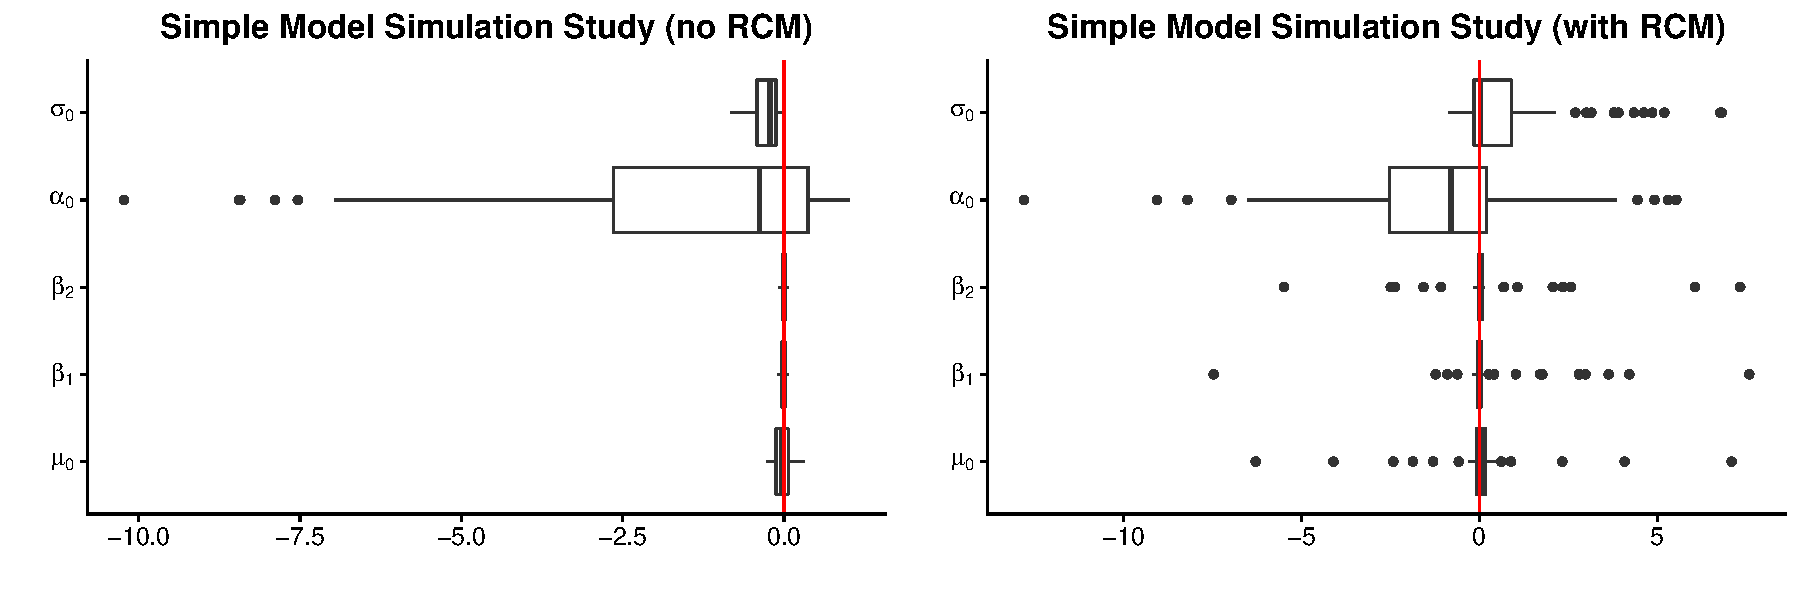
\includegraphics[width=12cm]{images/fitting/simple_model/ss_boxplots.pdf}
        \caption{Model $\mathcal{B}$ Simulation Study Box Plots}
        \label{fig:ss-simple}
\end{figure}

\begin{table}[H]
\caption{Root Mean Squared Errors for Model $\mathcal{B}$}
\label{tab:rmse-simple}
\begin{tabular}{@{}lll@{}}
\toprule
Parameter & RMSE without RCM ($3$ s.f.) & RMSE with RCM ($3$ s.f.) \\ \midrule
$\mu_0$   & 0.126                    & 1.69                  \\
$\beta_1$ & 0.0366                   & 1.85                  \\
$\beta_2$ & 0.0352                   & 1.76                  \\
$\tau_{\alpha_0}$ & 3.42                     & 3.79                  \\
$\tau_{\sigma_0}$ & 0.353                    & 2.23                  \\ \bottomrule
\end{tabular}
\end{table}

The results show that Synthetic Likelihood Estimation, both with and without the Robust Covariance Matrix can achieve convergence to the true parameters. Notably, using the Robust Covariance Matrix increases the RMSE and the number of outliers, this is to be expected since it is a noisy estimator. However, as will be seen when looking at the performance, the Robust Covariance Matrix runs much more quickly. Thus, the observation length can be increased far past what would be computationally reasonable when not using the Robust Covariance Matrix. This itself can significantly should reduce the RMSE due to the asymptotic normality of the $M$-Estimator (Thereom~\ref{the:aymp}).

\subsubsection{Performance}
\label{subsec:perf}

Moving on to performance. This can be analysed by repeatedly timing how long it takes to evaluate a Synthetic Likelihood with and without the Robust Covariance Matrix. In this case, the Synthetic Likelihood of the true parameters (Table~\ref{tab:uk-val}) were evaluated using the R library \emph{microbenchmark}. In Figure~\ref{fig:ss-perf}, violin plots of the evaluation times are shown. The numerical Robust Covariance Matrix is evaluated using the `fdHess' function from the R library \emph{nlme}. It is clear that the Robust Covariance Matrix provides a significant performance boost. Specifically, the median time when not using the Robust Covariance Matrix was $6$ms, about $37\times$ longer than $0.16\text{ms}$, the median time when using the Analytic Robust Covariance Matrix. Additionally, not using the Robust Covariance Matrix takes about $7\times$ longer than $0.87\text{ms}$, the median time when using the Numerical Robust Covariance Matrix. Thus, including the Robust Covariance Matrix with a numerical Hessian estimate significantly improves computational performance. However, the bulk of the computational performance improvement comes when using an analytic Hessian.

\begin{figure}[H]
        \centering
        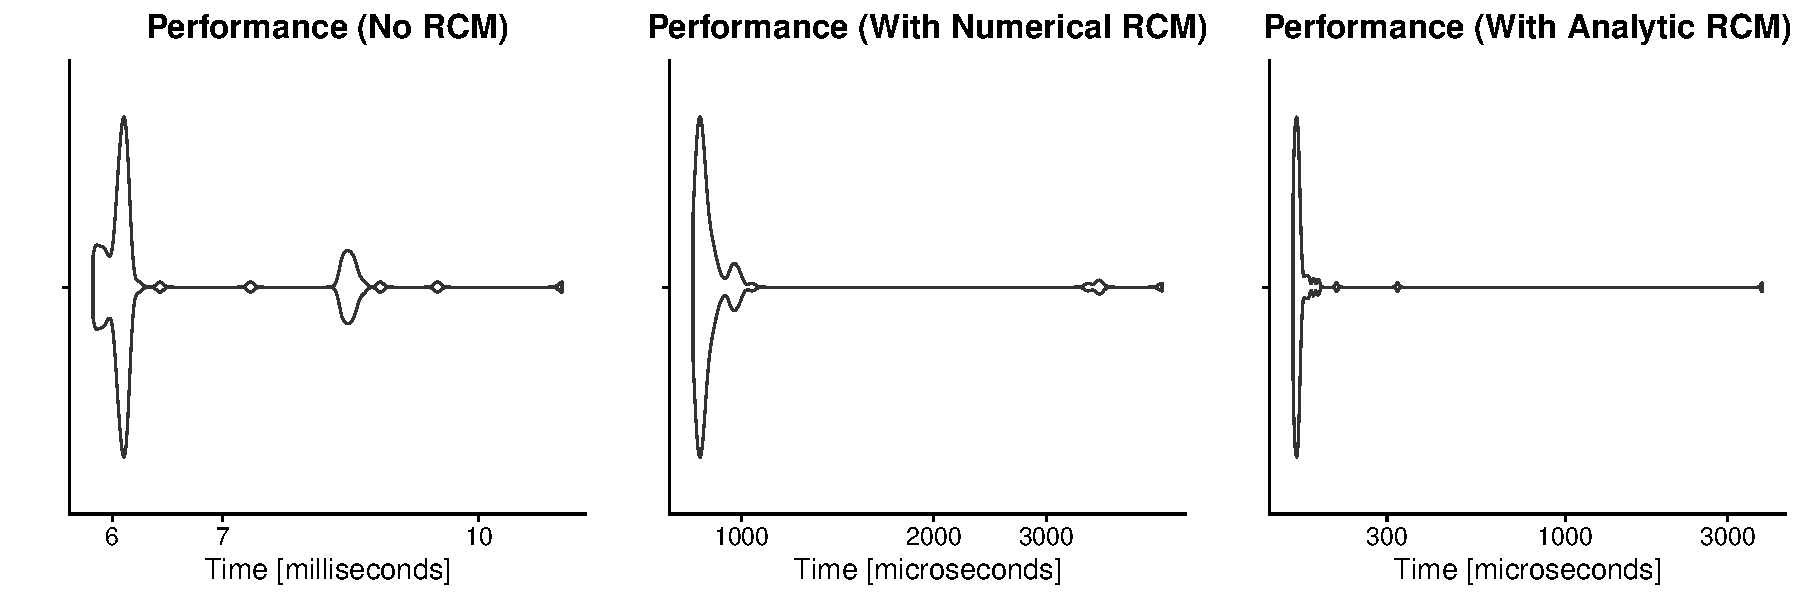
\includegraphics[width=12cm]{images/fitting/simple_model/perf.pdf}
        \caption{Comparative Performance of Robust Covariance Matrix}
        \label{fig:ss-perf}
\end{figure}

This section has demonstrated how using the Robust Covariance Matrix can be used within Synthetic Likelihood Estimation to provide significant computational benefit.

The next section will address fitting Model $\mathcal{A}$.

\subsection{Fitting Model \texorpdfstring{$\mathcal{A}$}{A}}
\label{subsec:fit-full-model}

\subsubsection{Choice of Statistics}
\label{subsec:full-stats}

Now that Model $\mathcal{B}$ has been successfully fit, it is time to return to the Model $\mathcal{A}$. Statistics need to be chosen that capture the nature of all parameters. For clarity, the parameters will be split up into the following groups. The weekly shape parameters: $\mu_0, \beta_1$ and $\beta_2$. The volatility parameters: $\sigma_0, \sigma_1$ and $\sigma_{-1}$. The mean reversion parameters: $\alpha_0$ and $\alpha_{-1}$. Finally, the spike parameters: $\mu_1$ and $p$.

To fit the Model $\mathcal{A}$, statistics will need to be chosen that are not $M$-estimators. Future projects may try to find equivalent $M$-estimators.

Before diving into the individual parameters, as shown in \cite{wood_2010}, including statistics that quantify the `shape of the marginal distribution' can be useful. These can be obtained as the coefficients of the polynomial regression between the ordered differences of the simulated trajectory and the observed trajectory. Ordered differences means the differences $y_{i+1} - y_i$ ordered from smallest to largest. This proves to be a good way to ensure the trajectories produced from fitted parameters follow similar distributions to the distribution of the observed trajectory. This project will use cubic regression and denote the coefficients $\gamma_0(\cdot), \gamma_1(\cdot), \gamma_2(\cdot), \gamma_3(\cdot)$.

For the shape parameters, similar statistics to those chosen for Model $\mathcal{B}$ can be used. For example, for $\mu_0$, the sample mean denoted $\bar{x}(\cdot)$, can be used. For $\beta_1$, the sample mean taken over Saturdays minus the sample mean can be used. This can be written as $(\bar{x}_5 - \bar{x})(\cdot)$. Subtracting the sample mean reduces the correlation between this statistic and the sample mean which will improve the Synthetic Likelihood Estimate. Similarly, $\beta_2$ can be inferred from $(\bar{x}_6 - \bar{x})(\cdot)$.

There are several statistics that provide useful information about the volatility parameters. Most obviously, the sample standard deviation, denoted $\sd{(\cdot)}$, and the interquartile range, denoted $\iqr{(\cdot)}$. However, the maximum of the absolute values of the trajectory will also exhibit some correlation with these parameters. Additionally, first and second order differences may also be of interest. That is, trajectory $\pmb{d}^1$ can be formed by $d^1_i = y_{i+1} - y_i$ and trajectory $\pmb{d}^2$ by $d^2_i = d_{i+1} - d_i$. Then, summary statistics for the distributions of $\pmb{d}^1$ and $\pmb{d}^2$ can be considered. Concretely, statistics such as the sample mean, standard deviation, skew and kurtosis can be calculated for $\pmb{d}^1$ and $\pmb{d}^2$. The sample skew shall be denoted as $\skewness{(\cdot)}$ and sample kurtosis as $\kurt{(\cdot)}$.

Another statistic that may be of interest for the volatility parameters is the maximum absolute difference, denoted $\max{|\cdot|}$. This statistic can be calculated for $\pmb{y}, \pmb{d}^1$ and $\pmb{d}^2$.

Now for the mean reversion parameters. Again, there are multiple approaches. As with Model $\mathcal{B}$, autoregression coefficients can be used. To account for the regime changing dynamics, it makes sense to regress on the past three days. The regression coefficients will be denoted $\xi_0(\cdot), \xi_1(\cdot), \xi_2(\cdot)$ and $\xi_3(\cdot)$. Additionally, autocorrelation coefficients up to lag 3 can also be explored, these will be denoted $\nu_0(\cdot), \nu_1(\cdot), \nu_2(\cdot)$ and $\nu_3(\cdot)$

Finally, the spike parameters $\mu_1$ and $p$ need to be considered. These parameters introduce skew to the trajectory distribution. Statistics that  measure skew include $\skewness{(\cdot)}$, the Maximum Likelihood Estimators for a Gamma distribution and the difference between the mean and median. The Maximum Likelihood Estimators for the Gamma distribution will be denoted $\theta_1(\cdot)$ and $\theta_2(\cdot)$ for the shape and rate parameters respectively. The median will be denoted $m(\cdot)$. Notably, since a Gamma distribution is defined for support $(0, \infty)$, the Maximum Likelihood Estimators will be evaluated for $(\exp(y_i), y_i \in \pmb{y})$, the exponentiated trajectory. 

Further, the spike parameters have similar effects to the volatility parameters, thus the statistics mentioned to capture those parameters are also of interest. However, even with all these statistics, it will still be difficult to get a good estimate of $p$, the probability of remaining in regime $0$. A statistic that is directly correlated with the frequency of the spikes is needed. To do this, the statistic denoted $\hat{p}(\cdot)$ will be constructed.

To construct $\hat{p}(\cdot)$, first notice the structure of the spikes. If there is a spike on day $i$, then the additional stochastic increment should increase the value $|d^1_{i-1}| = |y_i - y_{i-1}|$. However, volatility $\sigma_0$ could also cause this. The crucial element is on day $i+1$, the model will be in the reverting regime, so $|d^1_{i}| = |y_{i+1} - y_i|$ should also be large. This is shown in Figure~\ref{fig:spike-stat}. Thus, construct the spike series $\pmb{s}$ by $s_i = |d^1_{i-1}| + |d^1_i| $. To get an idea for the frequency of spikes, define $\hat{p}(\cdot)$ to be the number of elements $s_i$ of $\pmb{s}$, such that $s_i > \bar{x}(\pmb{s}) + 2\sd{(\pmb{s})}$. This statistic should provide high correlation with the frequency of the spikes, thus, demonstrate high correlation with $p$.

\subfile{spike_diagram}

These statistics can be investigated using the correlation diagrams from Section~\ref{subsec:corr_diag}. The results can be seen in Figure~\ref{fig:fmcd}.

\begin{figure}[H]
        \centering
        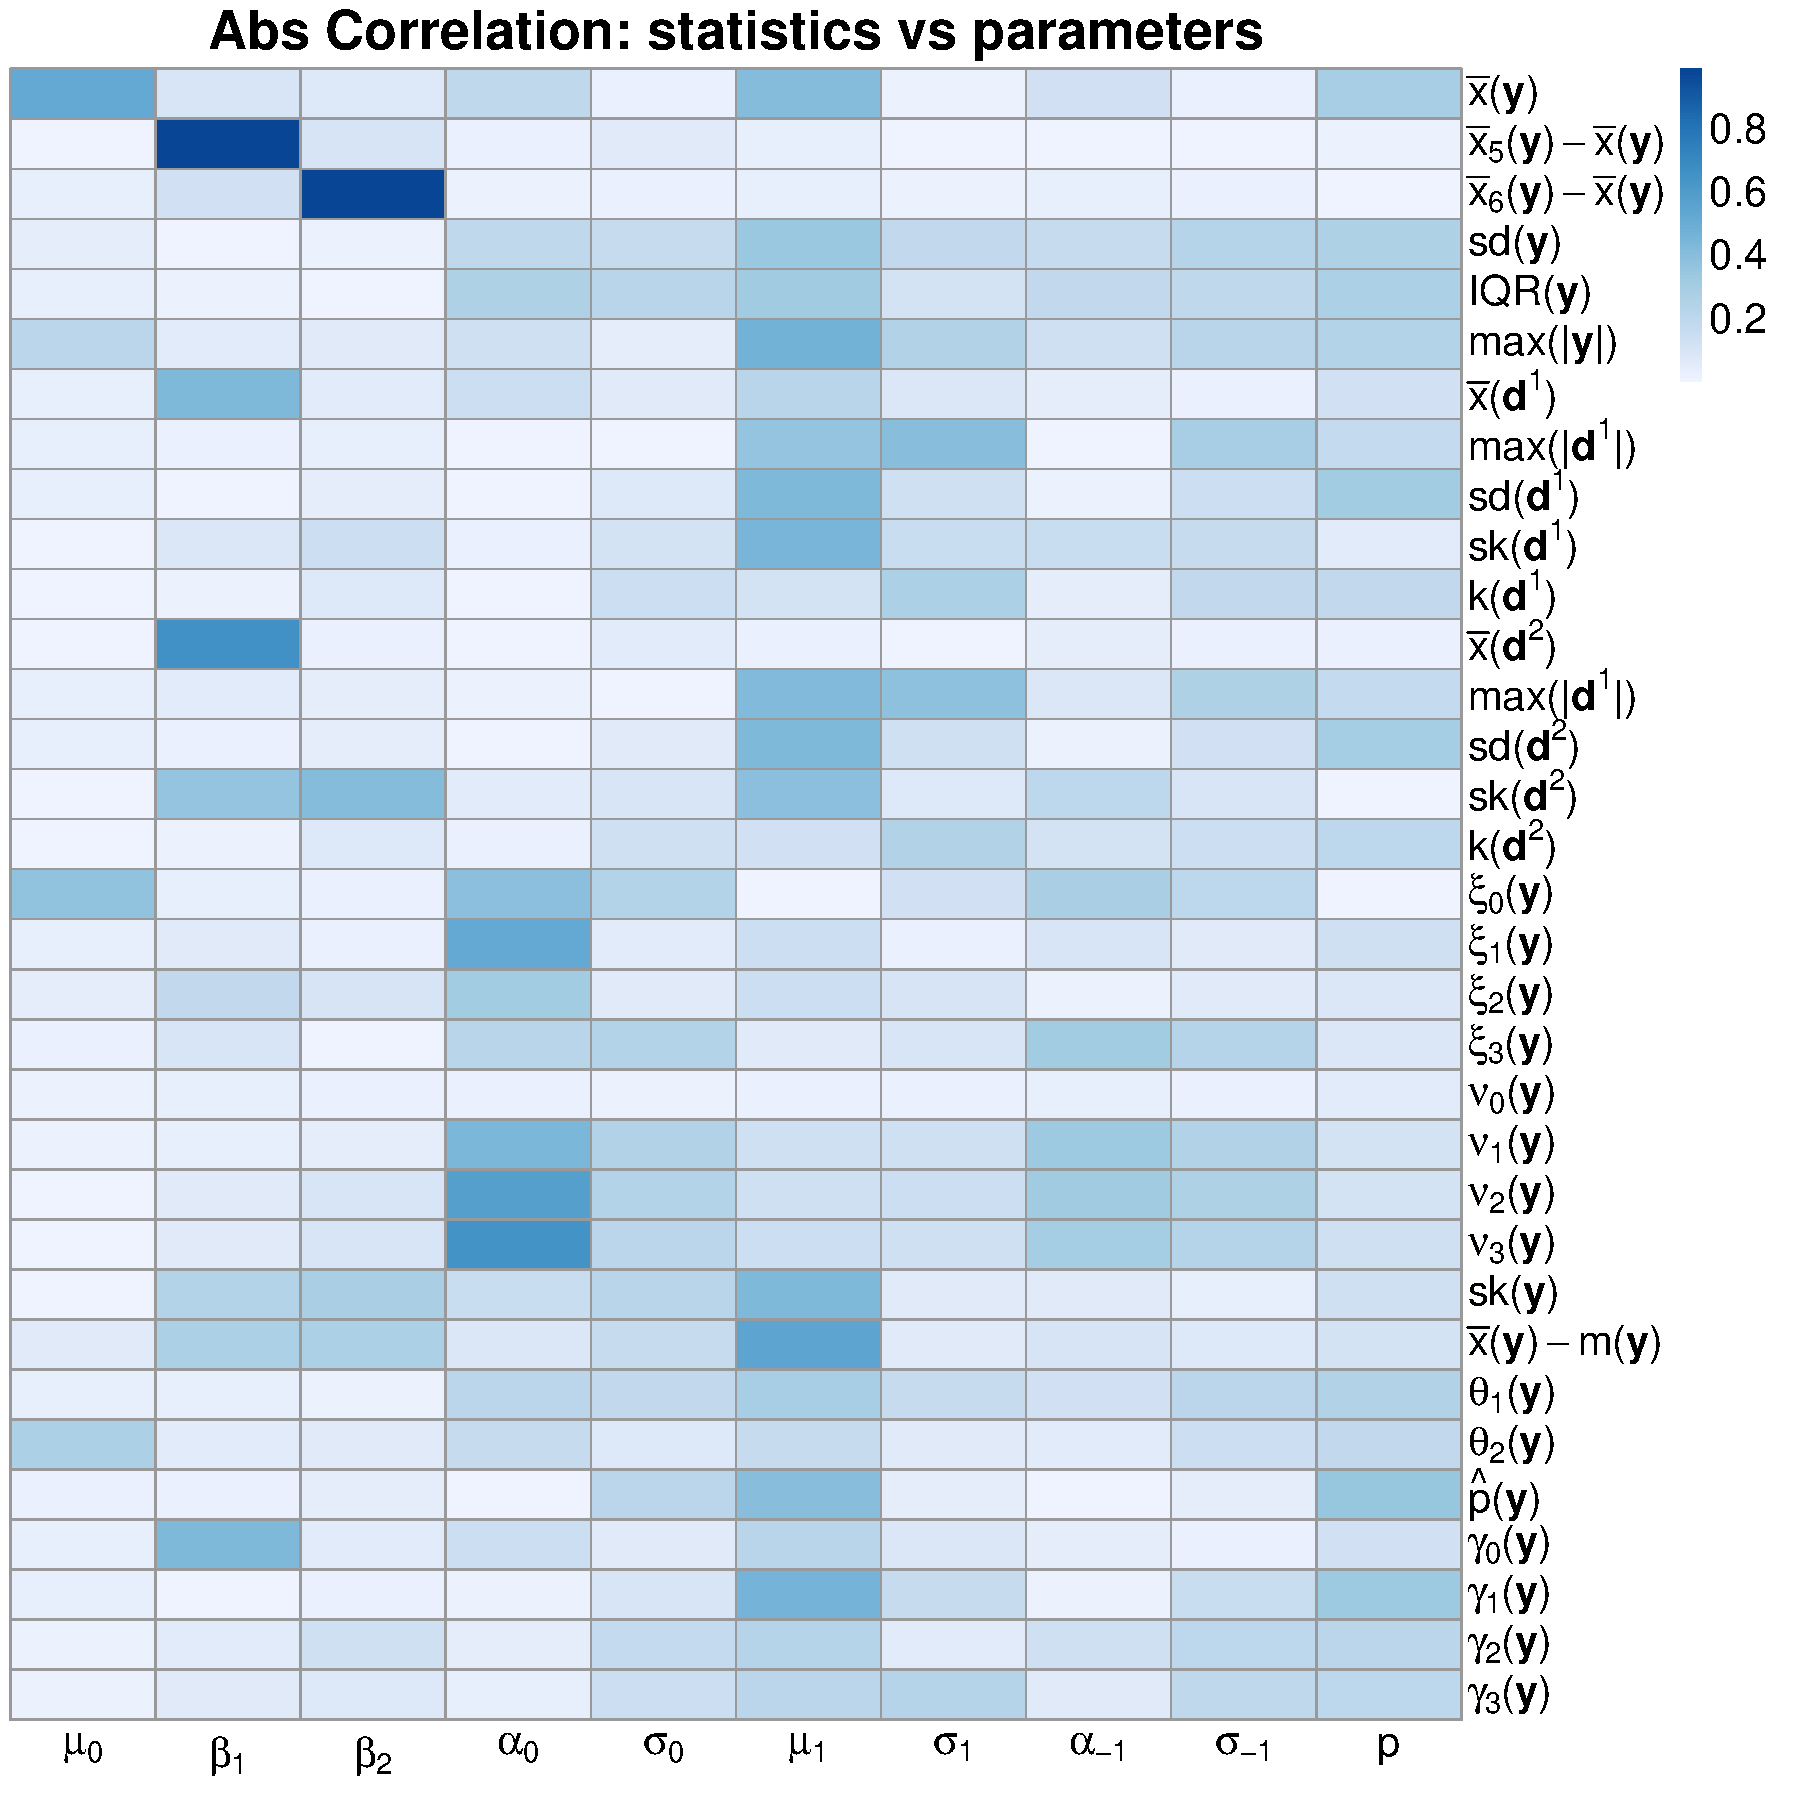
\includegraphics[width=95mm]{images/fitting/full_model/cor_sp.pdf}
        \vspace{1cm}
        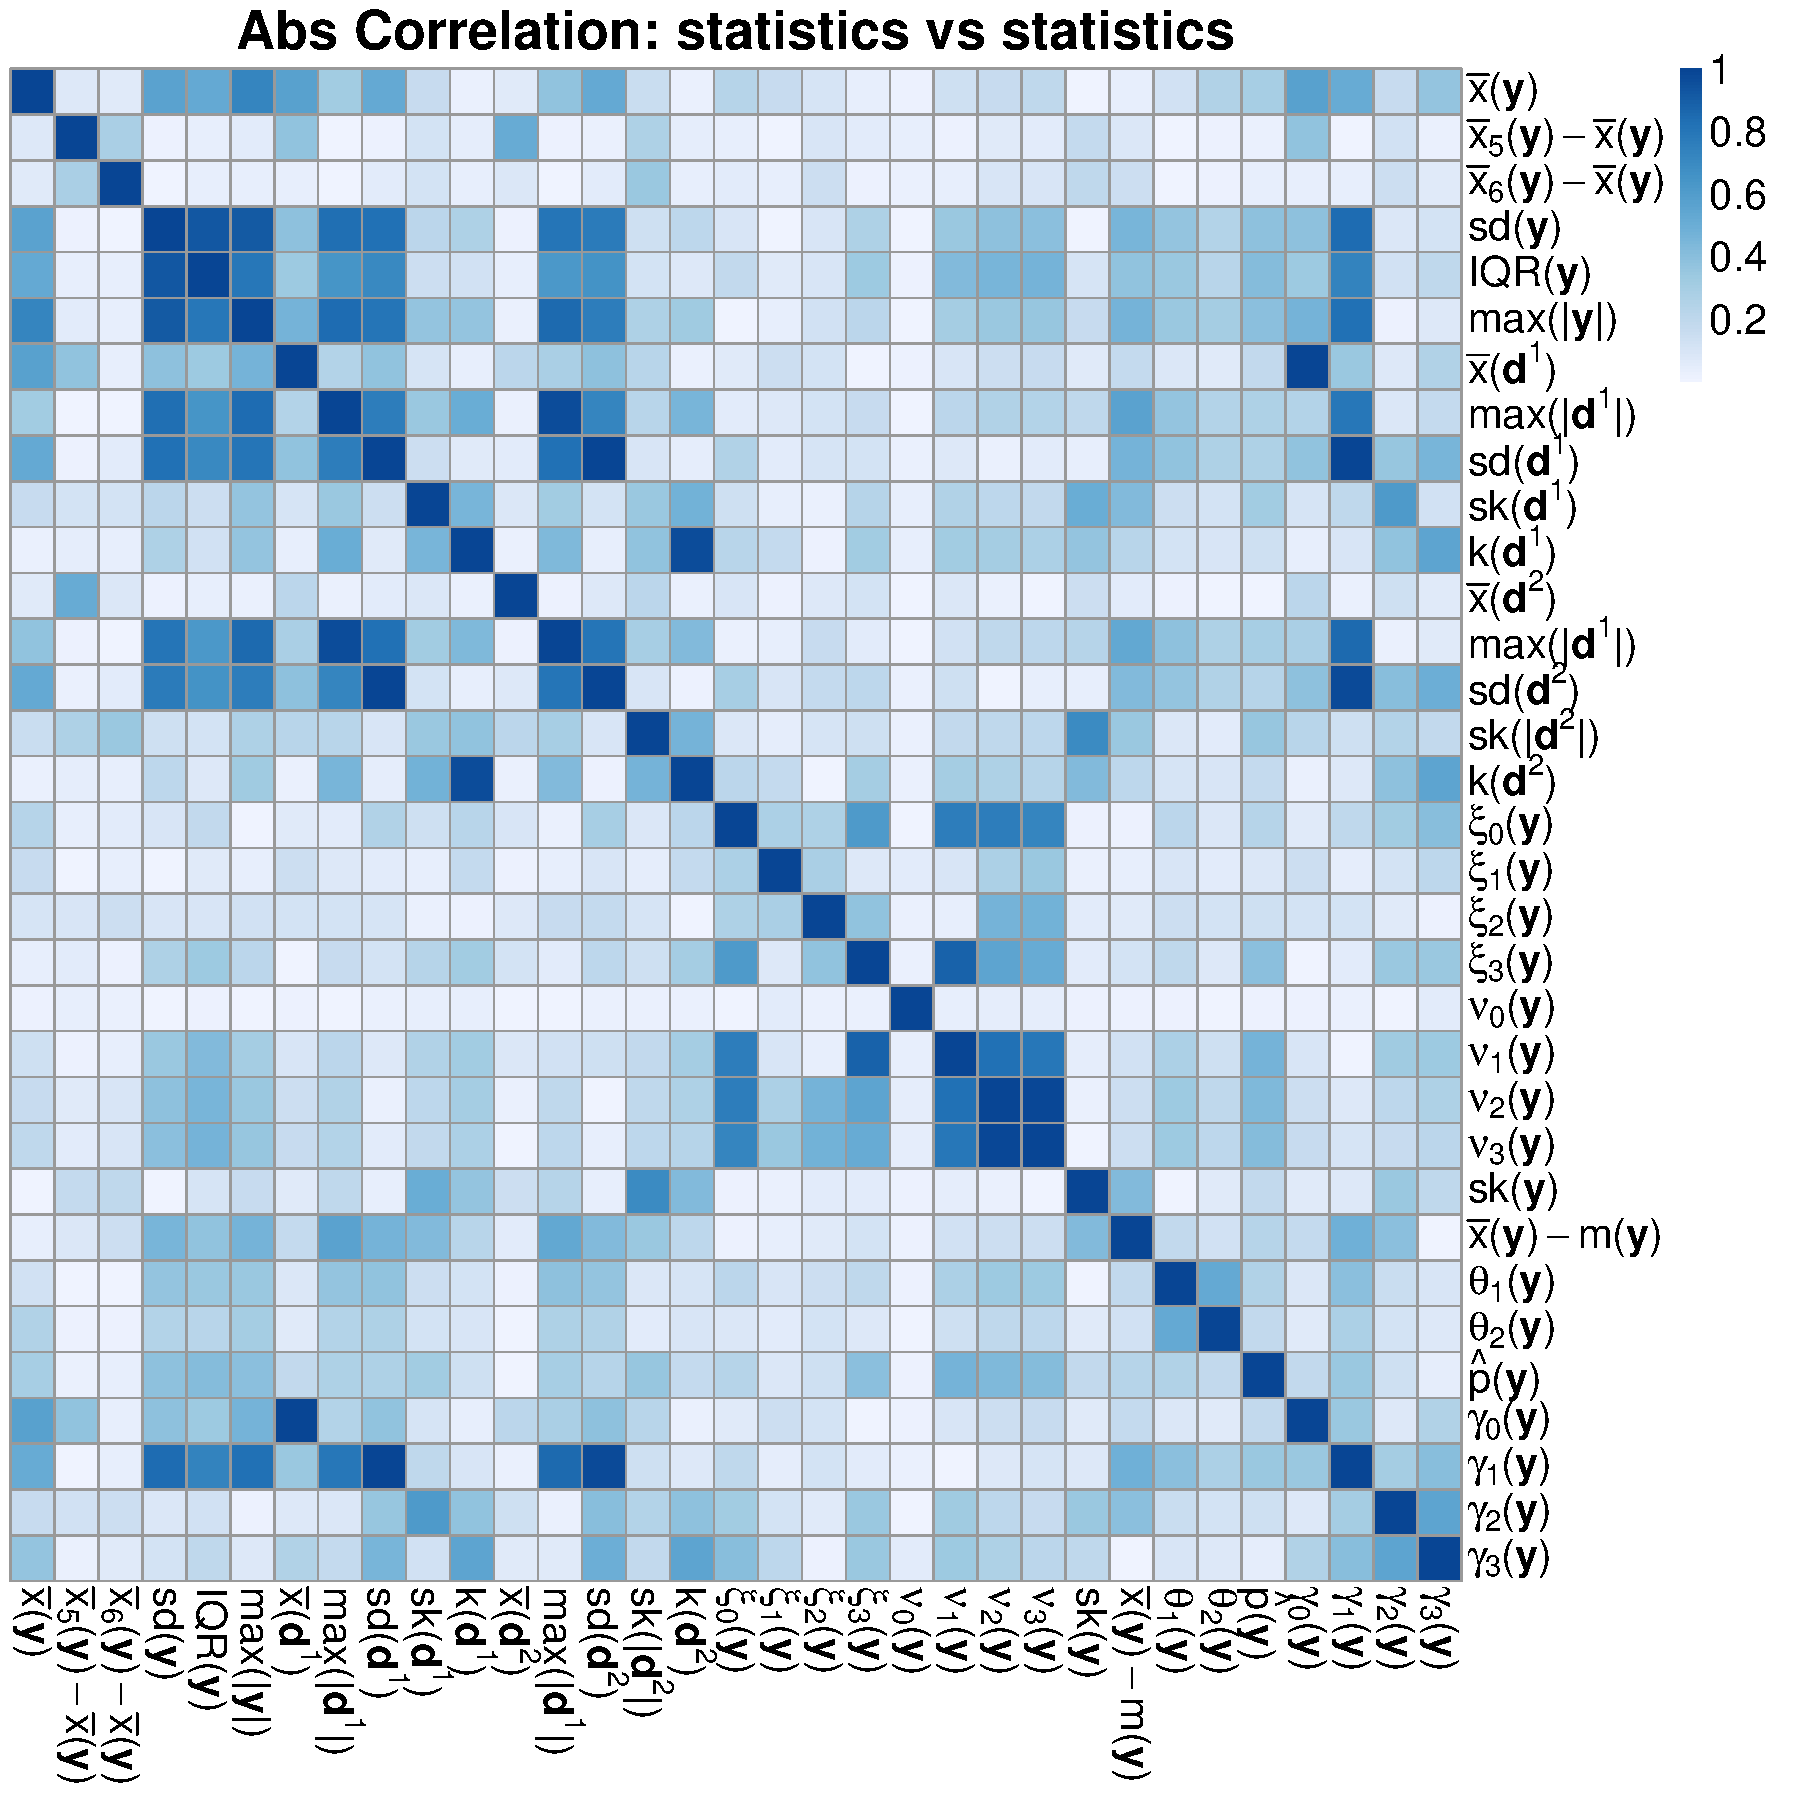
\includegraphics[width=95mm]{images/fitting/full_model/cor_ss.pdf}
        \caption{Model $\mathcal{A}$ Correlation Diagrams}
        \label{fig:fmcd}
\end{figure}

Most statistics can be removed due to either having not enough correlation with model parameters or too much correlation with other statistics. In particular, autoregression coefficients are favoured over autocorrelation coefficients due to their smaller mutual correlation, and all statistics based on the second order differences $\pmb{d}^2$ did not demonstrate enough correlation with model parameters to be included.

After some trial and improvement, $\bar{x}$, $\bar{x}_5 - \bar{x}$, $\bar{x}_6 - \bar{x}$, $\xi_1$, $\xi_3$, $\iqr{}$, $\max{|\pmb{d}^1|}$, $\max{|\pmb{y}|}$, $\hat{p}$, $\gamma_0$, $\gamma_1$, $\gamma_2$ and $\gamma_3$ were found, jointly, to be the best performing statistics.

Synthetic Likelihood Estimation can now be performed for Model $\mathcal{A}$. The next section will check for convergence to the true parameters.

\subsubsection{Checking Convergence}

Before proceeding with this section, one final adjustment needs to be made. Spike parameter $\mu_1$ needs to be replaced with the transformed parameter $\tau_{\mu_1}$ where $\mu_1 = \exp{\tau_{\mu_1}}$. This constrains $\mu_1$ to positive values. This is a useful constraint since the price spikes of interest are positive and negative spikes can upset the Synthetic Likelihood Estimation.

Now for the simulation study. Using the same process used for Model $\mathcal{B}$, a simulation study can be used to check for convergence to the true parameters (Table~\ref{tab:uk-val}). As before, $50$ simulations were conducted. Box plots of the results are found in Figure~\ref{fig:ss-full}; RMSE values are found in Table~\ref{tab:rmse-full}.

\begin{table}[H]
\caption{Root Mean Squared Errors for Model $\mathcal{A}$}
\label{tab:rmse-full}
\begin{tabular}{@{}lllllllllll@{}}
\toprule
\textbf{Parameter}: & $\mu_0$ & $\beta_1$ & $\beta_2$ & $\alpha_0$ & $\sigma_0$ & $\mu_1$ & $\sigma_1$ & $\alpha_{-1}$ & $\sigma_{-1}$ & $p$  \\
\midrule
\textbf{RMSE} ($3$ s.f.): & $0.177$   & $0.0631$    & $0.0560$    & $0.941$      & $3.75$      & $23.7$   & $4.14$      & $0.974$         & $6.29$         & $0.879$ \\
\bottomrule
\end{tabular}
\end{table}

\begin{figure}[H]
        \centering
        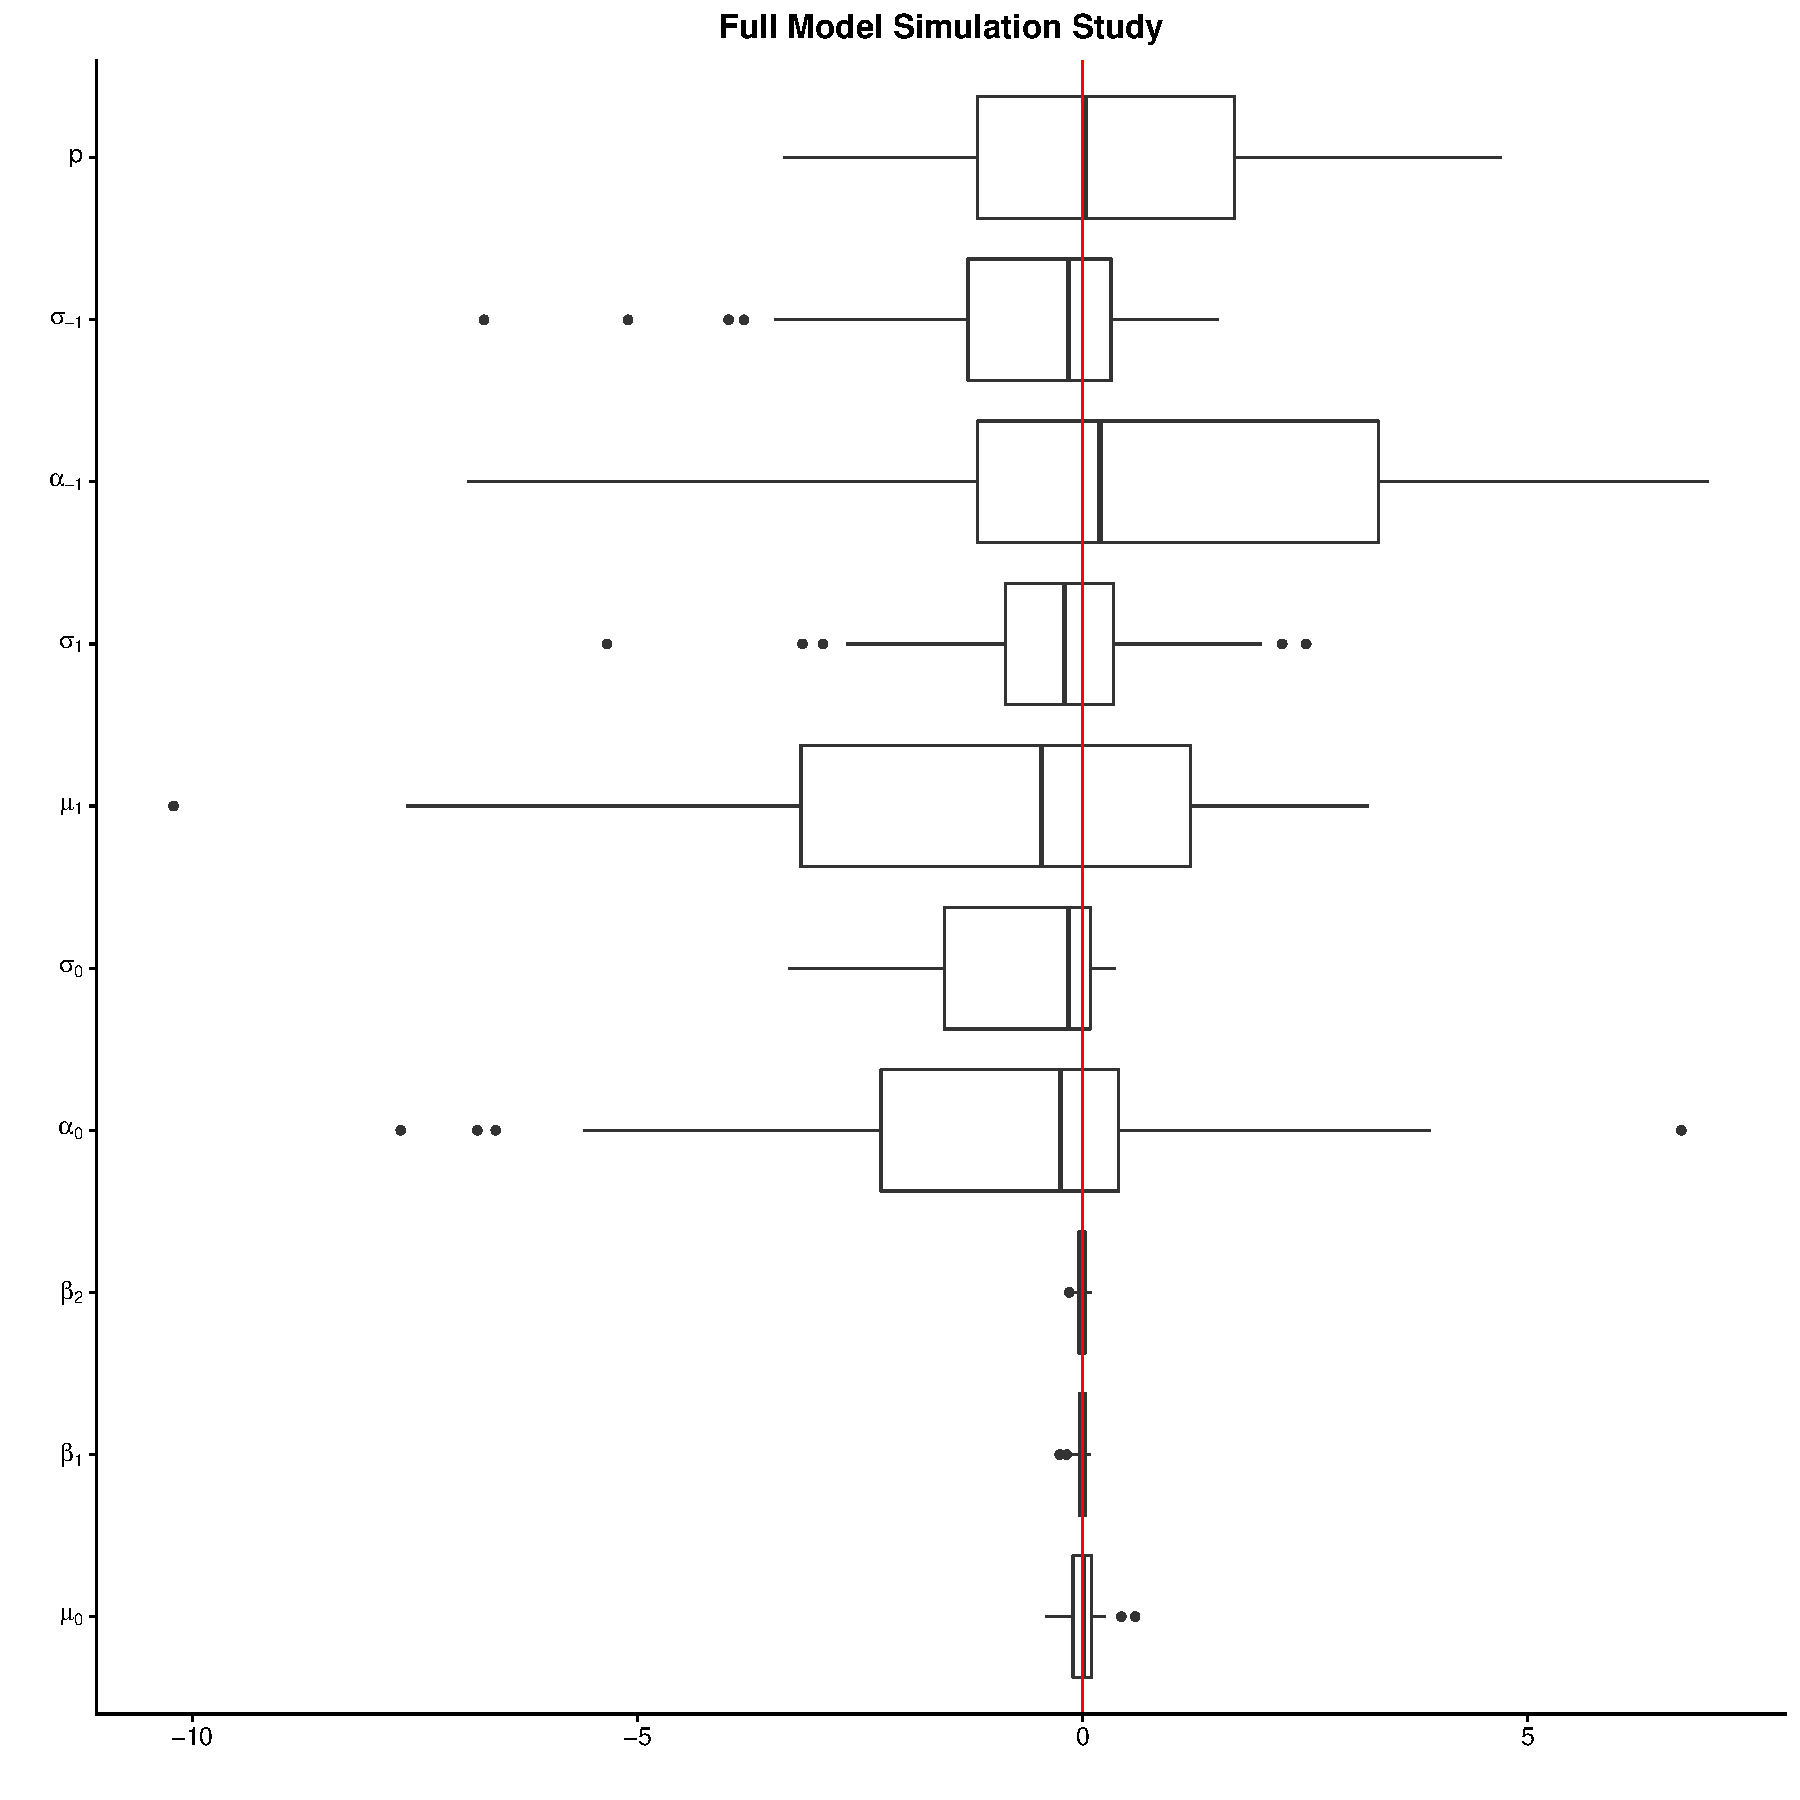
\includegraphics[width=10cm]{images/fitting/full_model/ss.pdf}
        \caption{Model $\mathcal{A}$ Simulation Study Box Plots}
        \label{fig:ss-full}
\end{figure}

All parameters converge around their true values. Since the simulation study only used an observation length of $100$, tighter fits with fewer outliers would be expected if the observation length was increased (Theorem~\ref{the:aymp}). The standout value for the RMSEs, is the value for $\tau_{\mu_1}$. This is partly since for an observation length of $100$ and a $p$ of $0.95$, there would only be approximately five spikes per simulation. This makes approximating the spike parameters a tall order that would be solved by using a longer observation length. This was not computationally feasible for this project.

Since the simulation study can provide strong evidence that the estimation will converge to the true parameters, the next section will cover fitting some real spot price data from Nordpool.

\subsubsection{Fitting With Nordpool Data}
\label{subsec:fit-real}

The data used for this project are the N2EX Day Ahead Auction Prices in GBP available from Nordpool's website.

Since Model $\mathcal{A}$ does not take seasonality into account, this project will look at spot prices for a particular season. Specifically, the log prices from Winter 2020 (October 2020 to March 2021) shown in Figure~\ref{fig:obs-traj}. There are two large spikes in the observed trajectory and maybe three or four smaller spikes. Once the model is fit, these spikes should be observed in the sampled trajectories.

\begin{figure}[H]
        \centering
        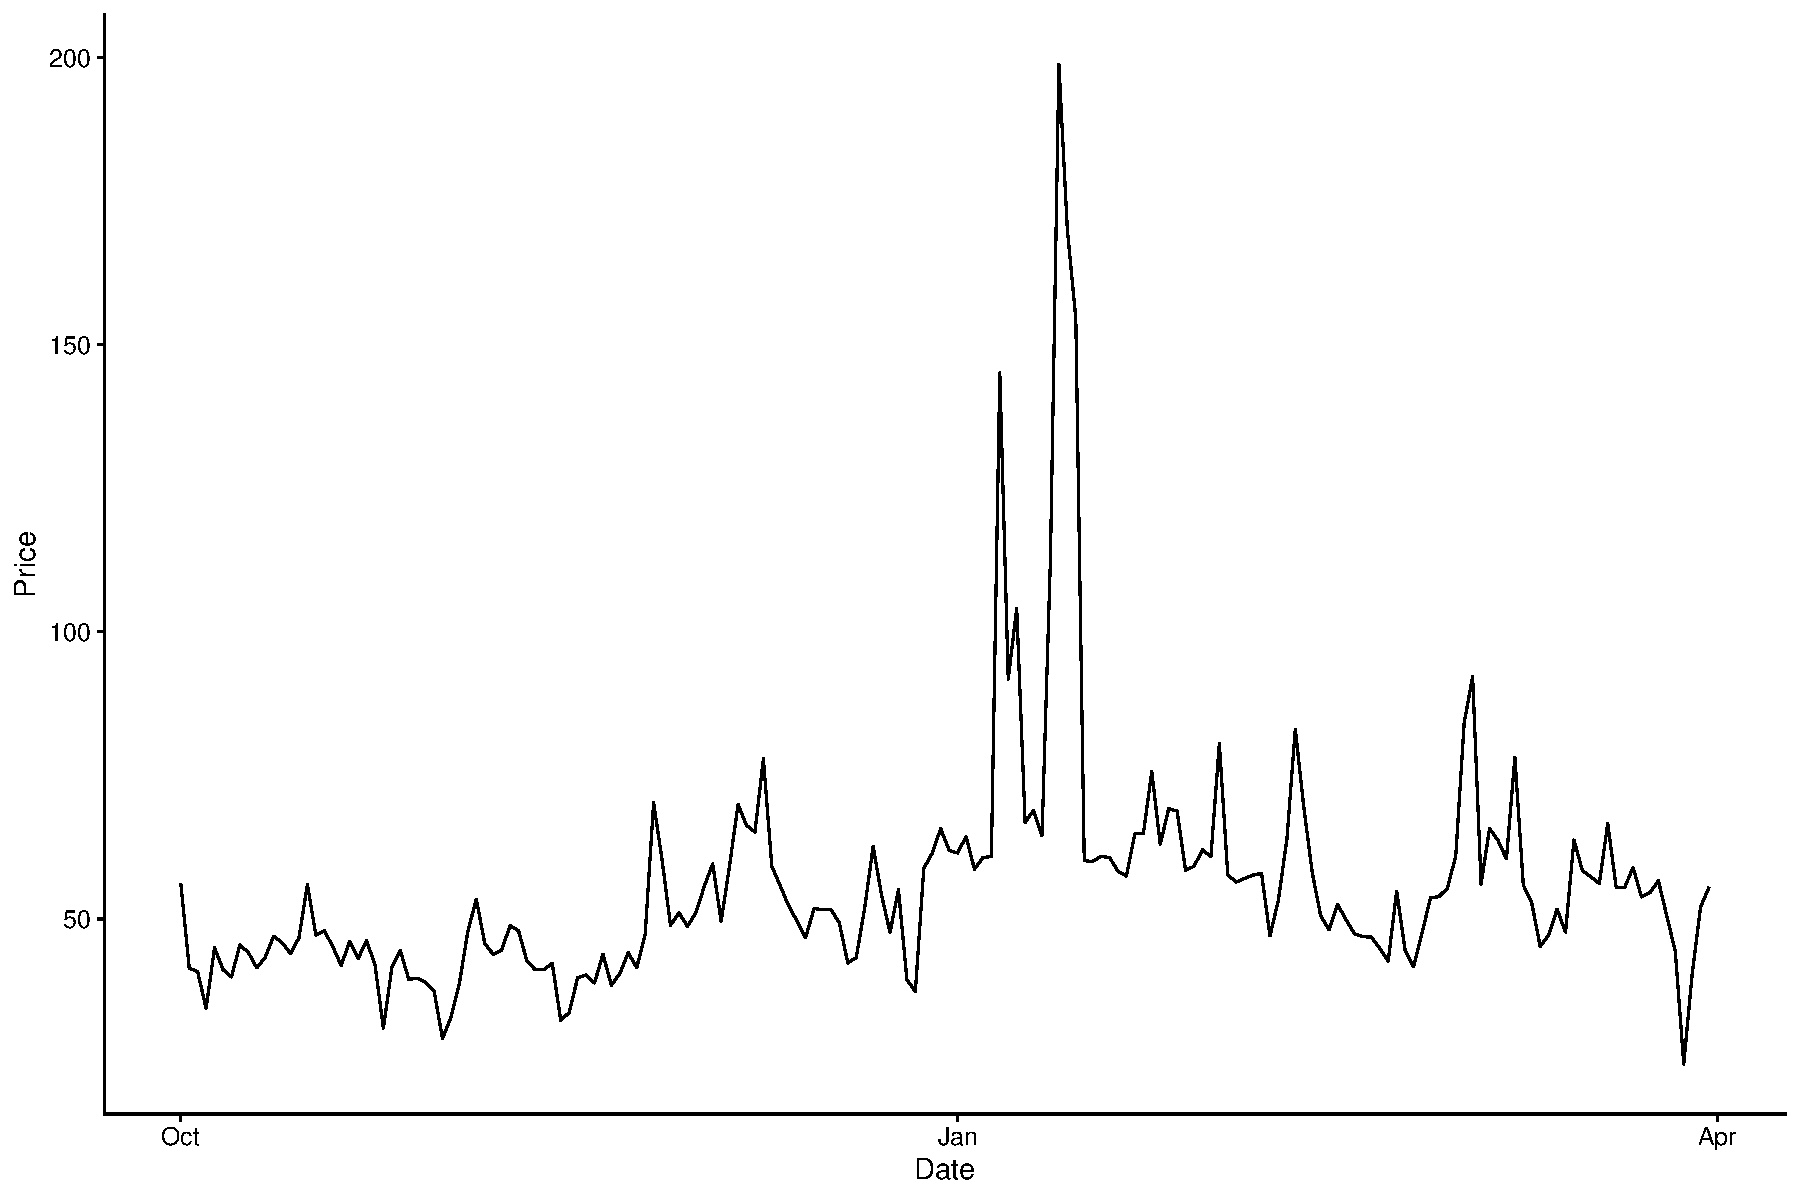
\includegraphics[width=12cm]{images/fitting/full_model/obs_traj.pdf}
        \caption{Observed Trajectory}
        \label{fig:obs-traj}
\end{figure}

In Table~\ref{tab:fitted-nordpool}, the initial and final parameter values are shown. The initial values were chosen by heuristic and from experience. For $\mu_0, \beta_1$ and $\beta_2$, samples means were used. For $\alpha_0$, a small amount of mean-reversion was included ($10\%$), for $\alpha_{-1}$ this was increased to $20\%$ to reflect that more mean-reversion would be expected after a spike compared to during regime $0$ (default price levels). For $\sigma_0$, a very small amount of volatility was included (0.05). This was increased to $0.5$ for during and after a spike ($\sigma_1$ and $\sigma_{-1}$ respectively). Finally, for the spike parameters, $\mu_1$ was set to $0.5$ to denote a small positive, but noticeable spike and $p$ was set to $0.995$ so that initially, the trajectory would remain, for the most part, in regime $0$.

\begin{table}[H]
\caption{Fitted Values for Nordpool Data}
\label{tab:fitted-nordpool}
\begin{tabular}{@{}lll@{}}
\toprule
Parameter & Initial Value ($3$ s.f.) & Final Value ($3$ s.f.) \\ \midrule
$\mu_0$   & $\bar{x}(\pmb{y}^0) = 3.97$ & $3.93$ \\
$\beta_1$ & $\bar{x}_5(\pmb{y}^0) - \bar{x}(\pmb{y}^0) = 0.0213$ & $0.0434$ \\
$\beta_2$ & $\bar{x}_6(\pmb{y}^0) - \bar{x}(\pmb{y}^0) = 0.095$ & $0.109$\\
$\tau_{\alpha_0}$ & $\log{\frac{0.1}{1-0.1}} = -2.20$ & $-1.01$ \\
$\tau_{\sigma_0}$ & $\log{0.05} = -3.00$ & $-2.13$ \\
$\tau_{\mu_1}$ & $\log{0.5} = -0.693$ & $-1.68$\\
$\tau_{\sigma_1}$ & $\log{0.5} = -0.693$ & $-2.15$ \\
$\tau_{\alpha_{-1}}$ & $\log{\frac{0.2}{1-0.2}} = -1.39$ & $1.66$ \\
$\tau_{\sigma_{-1}}$ & $\log{0.5} = -0.693$ & $-0.474$ \\
$\tau_{p}$ & $\log{\frac{0.995}{1-0.995}} = 5.29$ & $3.40$ \\ \bottomrule
\end{tabular}
\end{table}

A $\tau_{p}$ of $3.40$ corresponds to a $p$ of $0.97$. Since the trajectory length is $182$, around five spikes per sampled trajectory would be expected. This lines up nicely with the observed trajectory. However, the real test is if the sampled trajectories resemble the observed trajectory. Five sampled trajectories can be seen in Figure~\ref{fig:sim-traj}.

\begin{figure}[H]
        \centering
        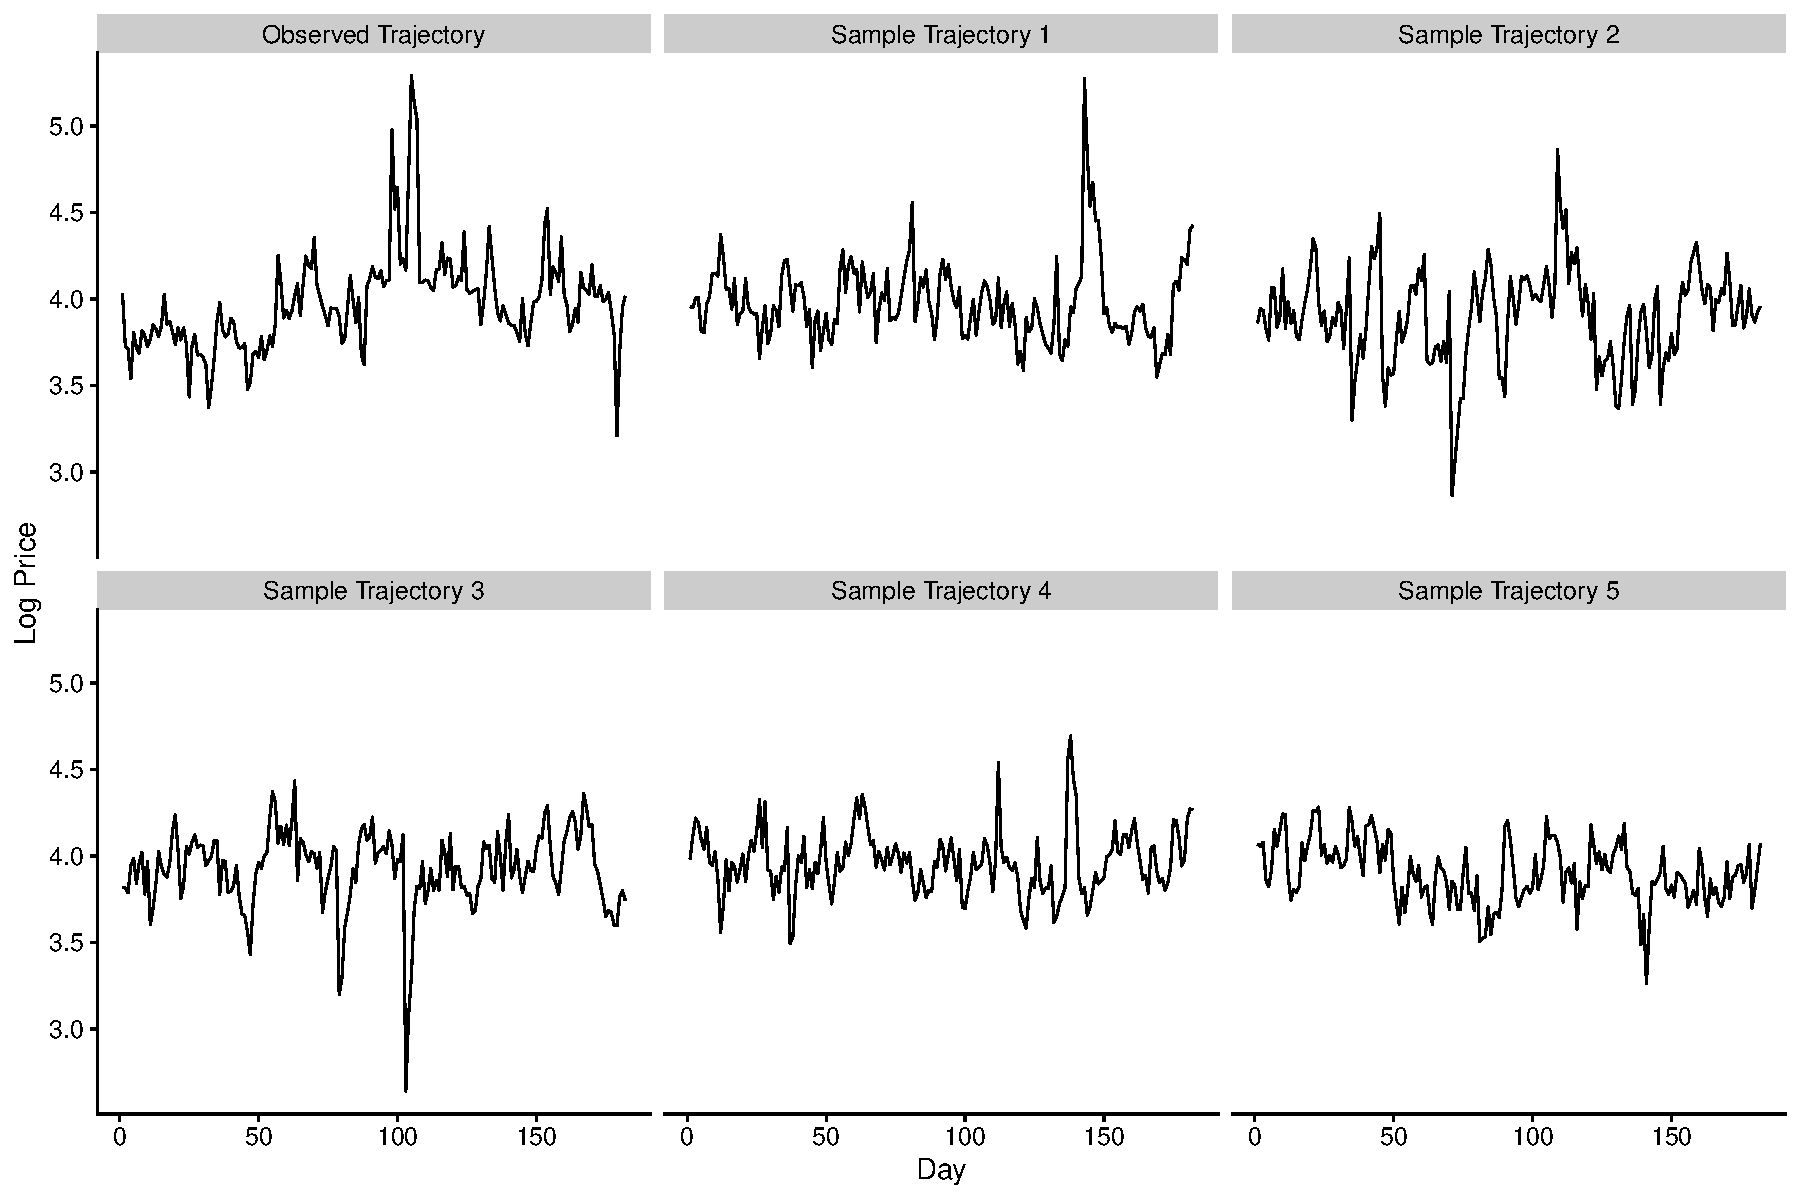
\includegraphics[width=12cm]{images/fitting/full_model/sim_traj.pdf}
        \caption{Simulated Trajectories}
        \label{fig:sim-traj}
\end{figure}

The trajectories match quite nicely in all but one aspect. The sampled trajectories have some negative spikes. This, as discussed in Section~\ref{sec:sl}, is a result of drawing the spikes from a Normal distribution. It should be noted that since the log price is being considered, these spikes will be less pronounced in the spot prices once the trajectories are exponentiated. Even so, this is an undesirable feature and modifying the model to eliminate these negative spikes presents an opportunity for future projects to explore.